%システム設計

本章では,SAS-L2を利用したセキュアな組込みシステムについての設計を述べる.
システム開発にあたり,基本設計の作成と役割分担,スケジュールの決定,詳細設計とテスト項目を作成した.
基本設計と詳細設計はUMLを用いて行った.

\section{基本設計}
基本設計では,ユースケース図とクラス図とシーケンス図を作成した.
\begin{figure}[H]
\begin{center}
	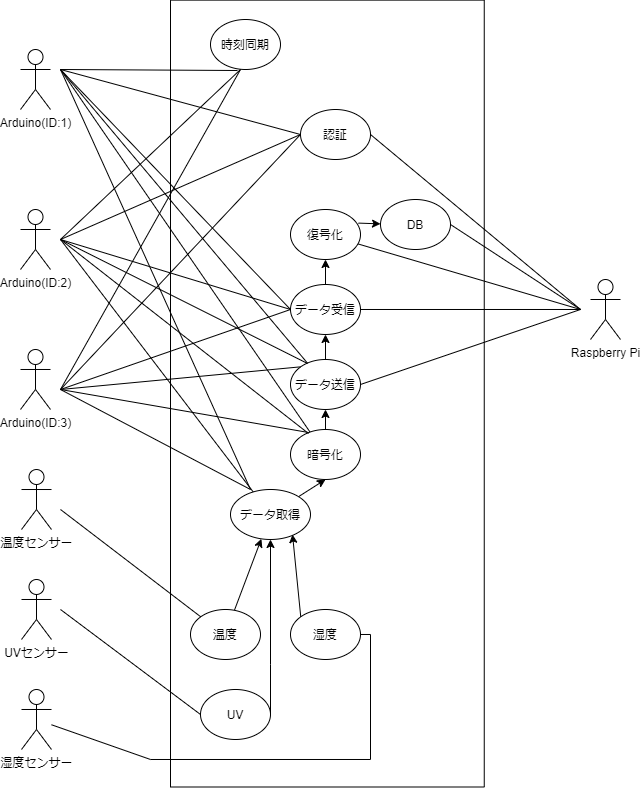
\includegraphics[width=10cm]{usecase.png}
	\caption{ユースケース図}
	\label{fig:kihon_usecase}
\end{center}
\end{figure}

図\ref{fig:kihon_usecase}のユースケース図では,システム内の基本機能を視覚的に図示している.
ユースケース図の作成により,システムの機能の洗い出しや役割分担を決定した.

\begin{figure}[H]
\begin{center}
	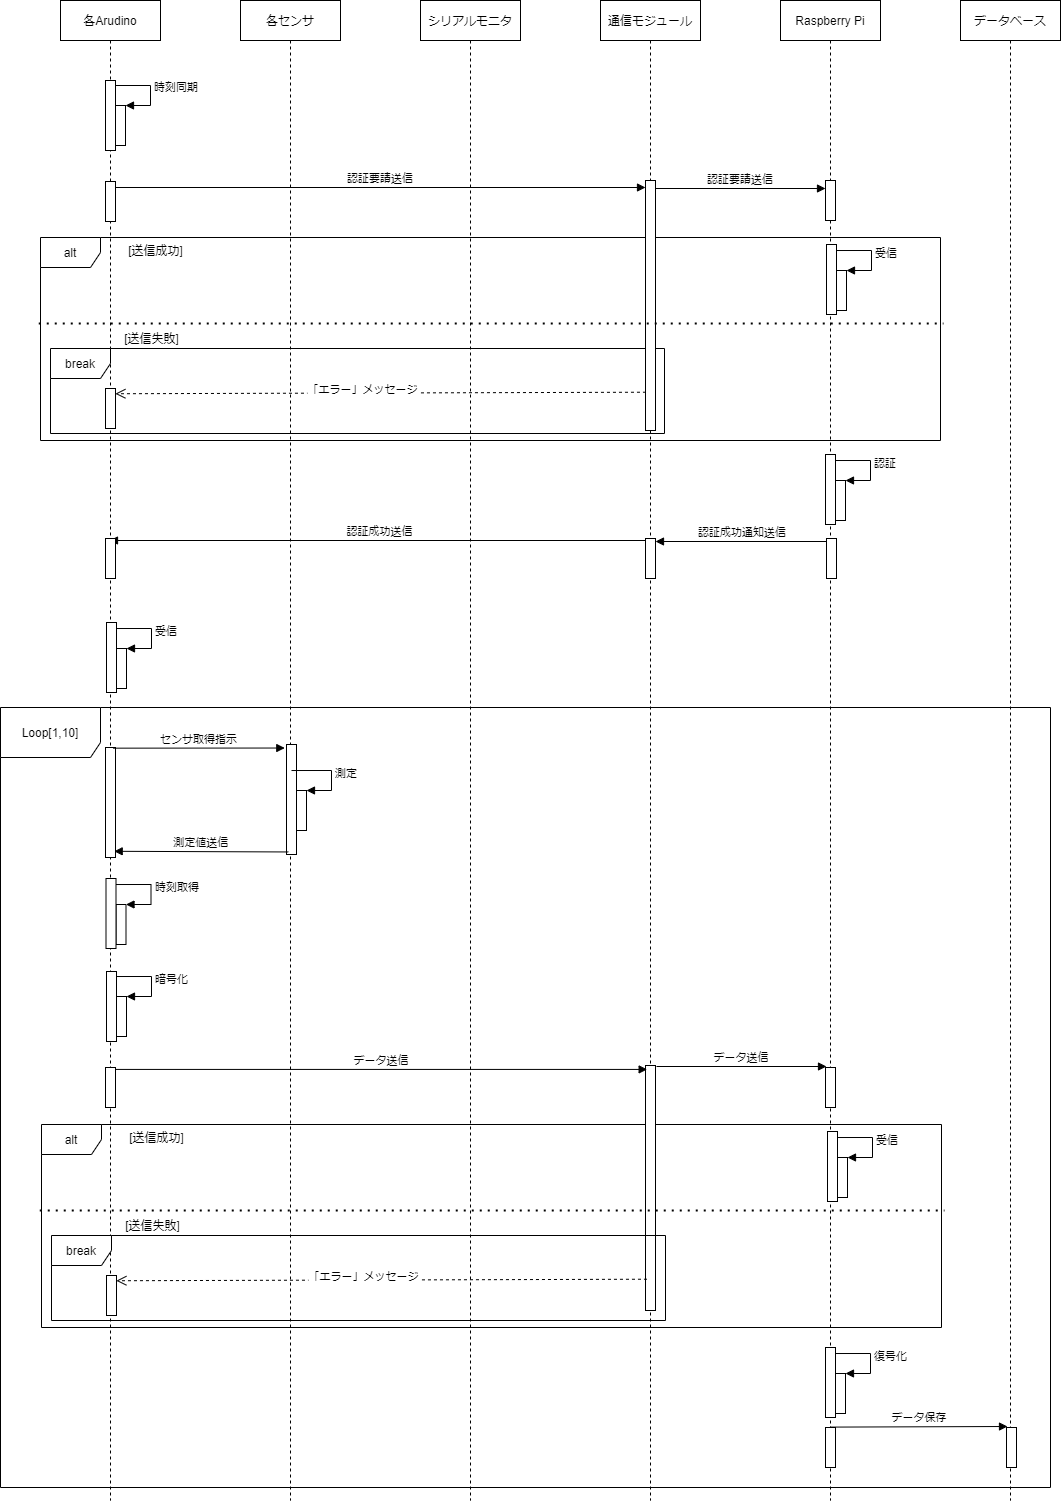
\includegraphics[height=200mm]{kihon_sequence.png}
	\caption{シーケンス図}
	\label{fig:kihon_sequence}
\end{center}
\end{figure}
図\ref{fig:kihon_sequence}のシーケンス図では,クラス間で行われる処理を時系列で表している.
初めに,Arduinoが時刻同期を行う.
次に,Arduinoから通信モジュールを経由してRaspbery Piへ認証要請を行う.
Arduinoが送信成功すればRaspbery Piは認証要請を受信し,送信失敗した場合は
通信モジュールからエラーメッセージが送信され,処理が中断される.
その後,Raspbery Piにより認証を行い,認証成功通知をArduinoへ送信する.
認証処理終了後,Arduinoは接続されているセンサからセンシングデータと,
センシングデータを取得した日時を取得し,暗号化を行う.
Arduinoは暗号化したデータをRaspbery Piへ送信し,
送信成功すればRaspbery Piはデータを受信し,送信失敗した場合は
通信モジュールからエラーメッセージが送信され,処理が中断される.
最後にRaspbery Piが受信したデータを復号し,得られたセンシングデータと
センシングデータの取得日時をデータベースへ保存する.
図\ref{fig:kihon_sequence}に示されているLoop[]はループと言い,[]内で示された範囲での繰り返し処理が行われる.
ここではLoop[1,10]であることから,10回の繰り返し処理が行われる.

\begin{figure}[H]
\begin{center}
	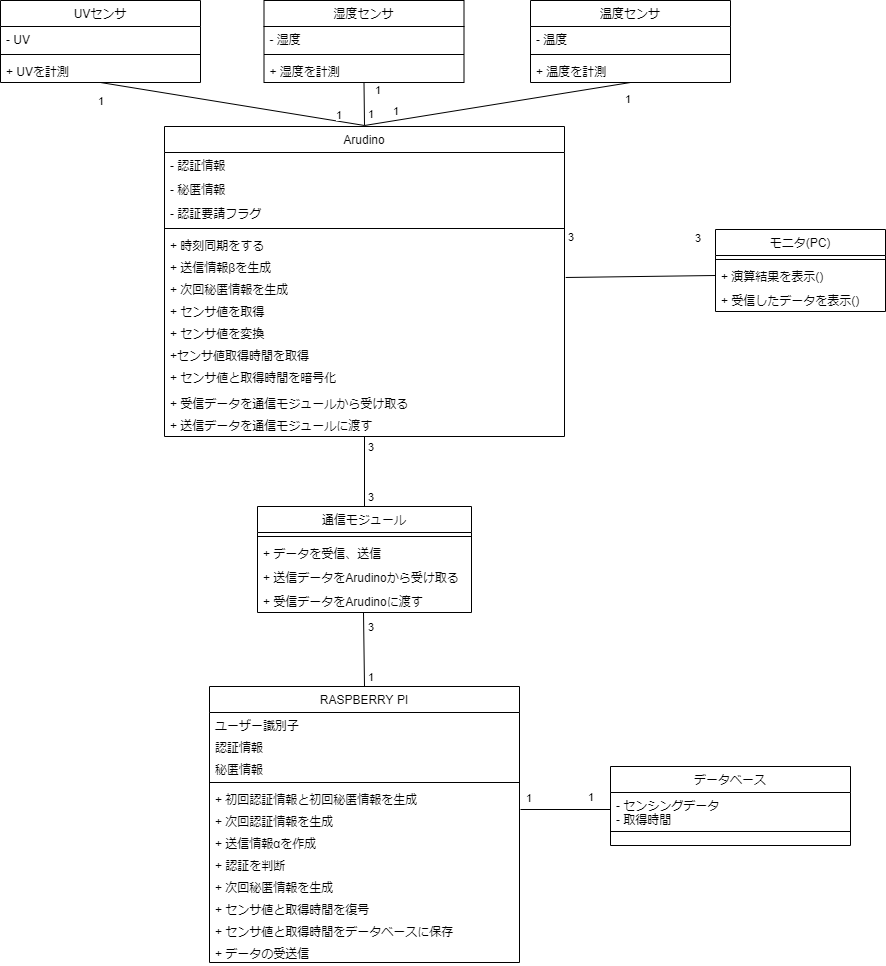
\includegraphics[height=140mm]{kihon_class.png}
	\caption{クラス図}
	\label{fig:kihon_class}
\end{center}
\end{figure}
図\ref{fig:kihon_class}のクラス図では,システムの静的な構造と関係性を視覚的に表している.
温度センサ,湿度センサ,UVセンサ,Arduino,モニタ,通信モジュール,Raspbery Pi,データベースをクラスとしている.
関連のあるクラス間での多重度も示している.

\section{役割分担}
図\ref{fig:kihon_usecase}のユースケース図から,役割分担を行った.
Arduinoの時刻同期とセンサからのセンシングデータ取得,データを暗号化しRaspbery Piへ送信する機能を浅野が担当した.
Raspbery PiのArduinoからのデータ受信とデータの復号化,データベースへの保存を内山田が担当した.
認証については,被認証側を浅野,認証側を内山田が担当した.

\section{スケジュール}
スケジュール管理は,ガントチャートで行った.
図\ref{fig:ganto}のようにガントチャートをEXCELで作成し,チーム内で共有しながら進捗を管理した.

\begin{figure}[H]
\begin{center}
	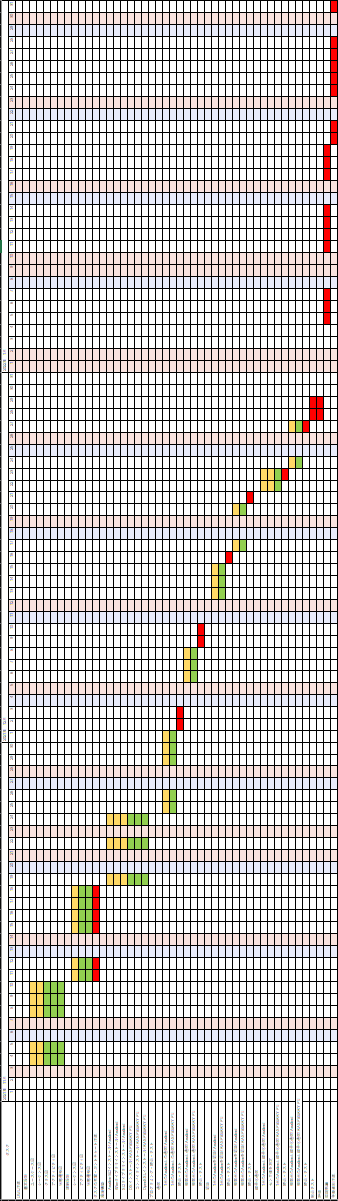
\includegraphics[height=220mm]{ganto.png}
	\caption{ガントチャート}
	\label{fig:ganto}
\end{center}
\end{figure}



\section{詳細設計}
担当する機能についての詳細設計をUMLを用いて行い,時間同期,認証における被認証者の処理,センシングデータの取得,暗号化通信についてのシーケンス図を作成した.
また,暗号化通信における通信フォーマットの定義も行った.

\begin{figure}[H]
\begin{center}
	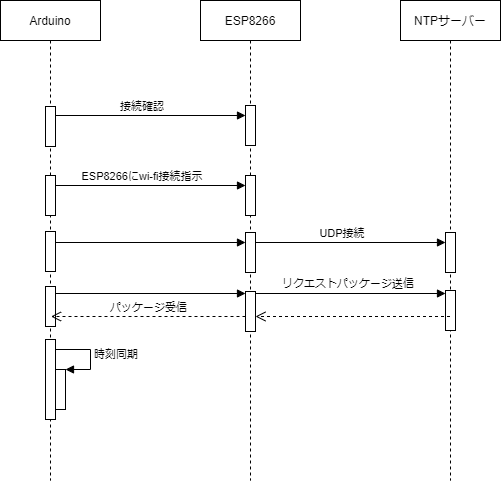
\includegraphics[height=80mm]{time_sequence.png}
	\caption{時間同期におけるシーケンス図}
	\label{fig:time_sequence}
\end{center}
\end{figure}
図\ref{fig:time_sequence}のシーケンス図では,Arduinoにおける時刻同期に関するクラス間で行われる処理を時系列で表している.
初めに,Arduinoが通信モジュールであるESP8266との接続を行う.
次に,Arduinoは通信モジュールを介してWi-Fiとの接続を行う.
日時を取得するために,ArduinoからNTPサーバーにUDP接続し,リクエストパッケージを送信する.
そして,NTPサーバーから受信したパッケージより,日時を取得して時刻同期を行う.
時刻同期の完了後,SAS-L2による認証・暗号化通信が行われる.

\begin{figure}[H]
\begin{center}
	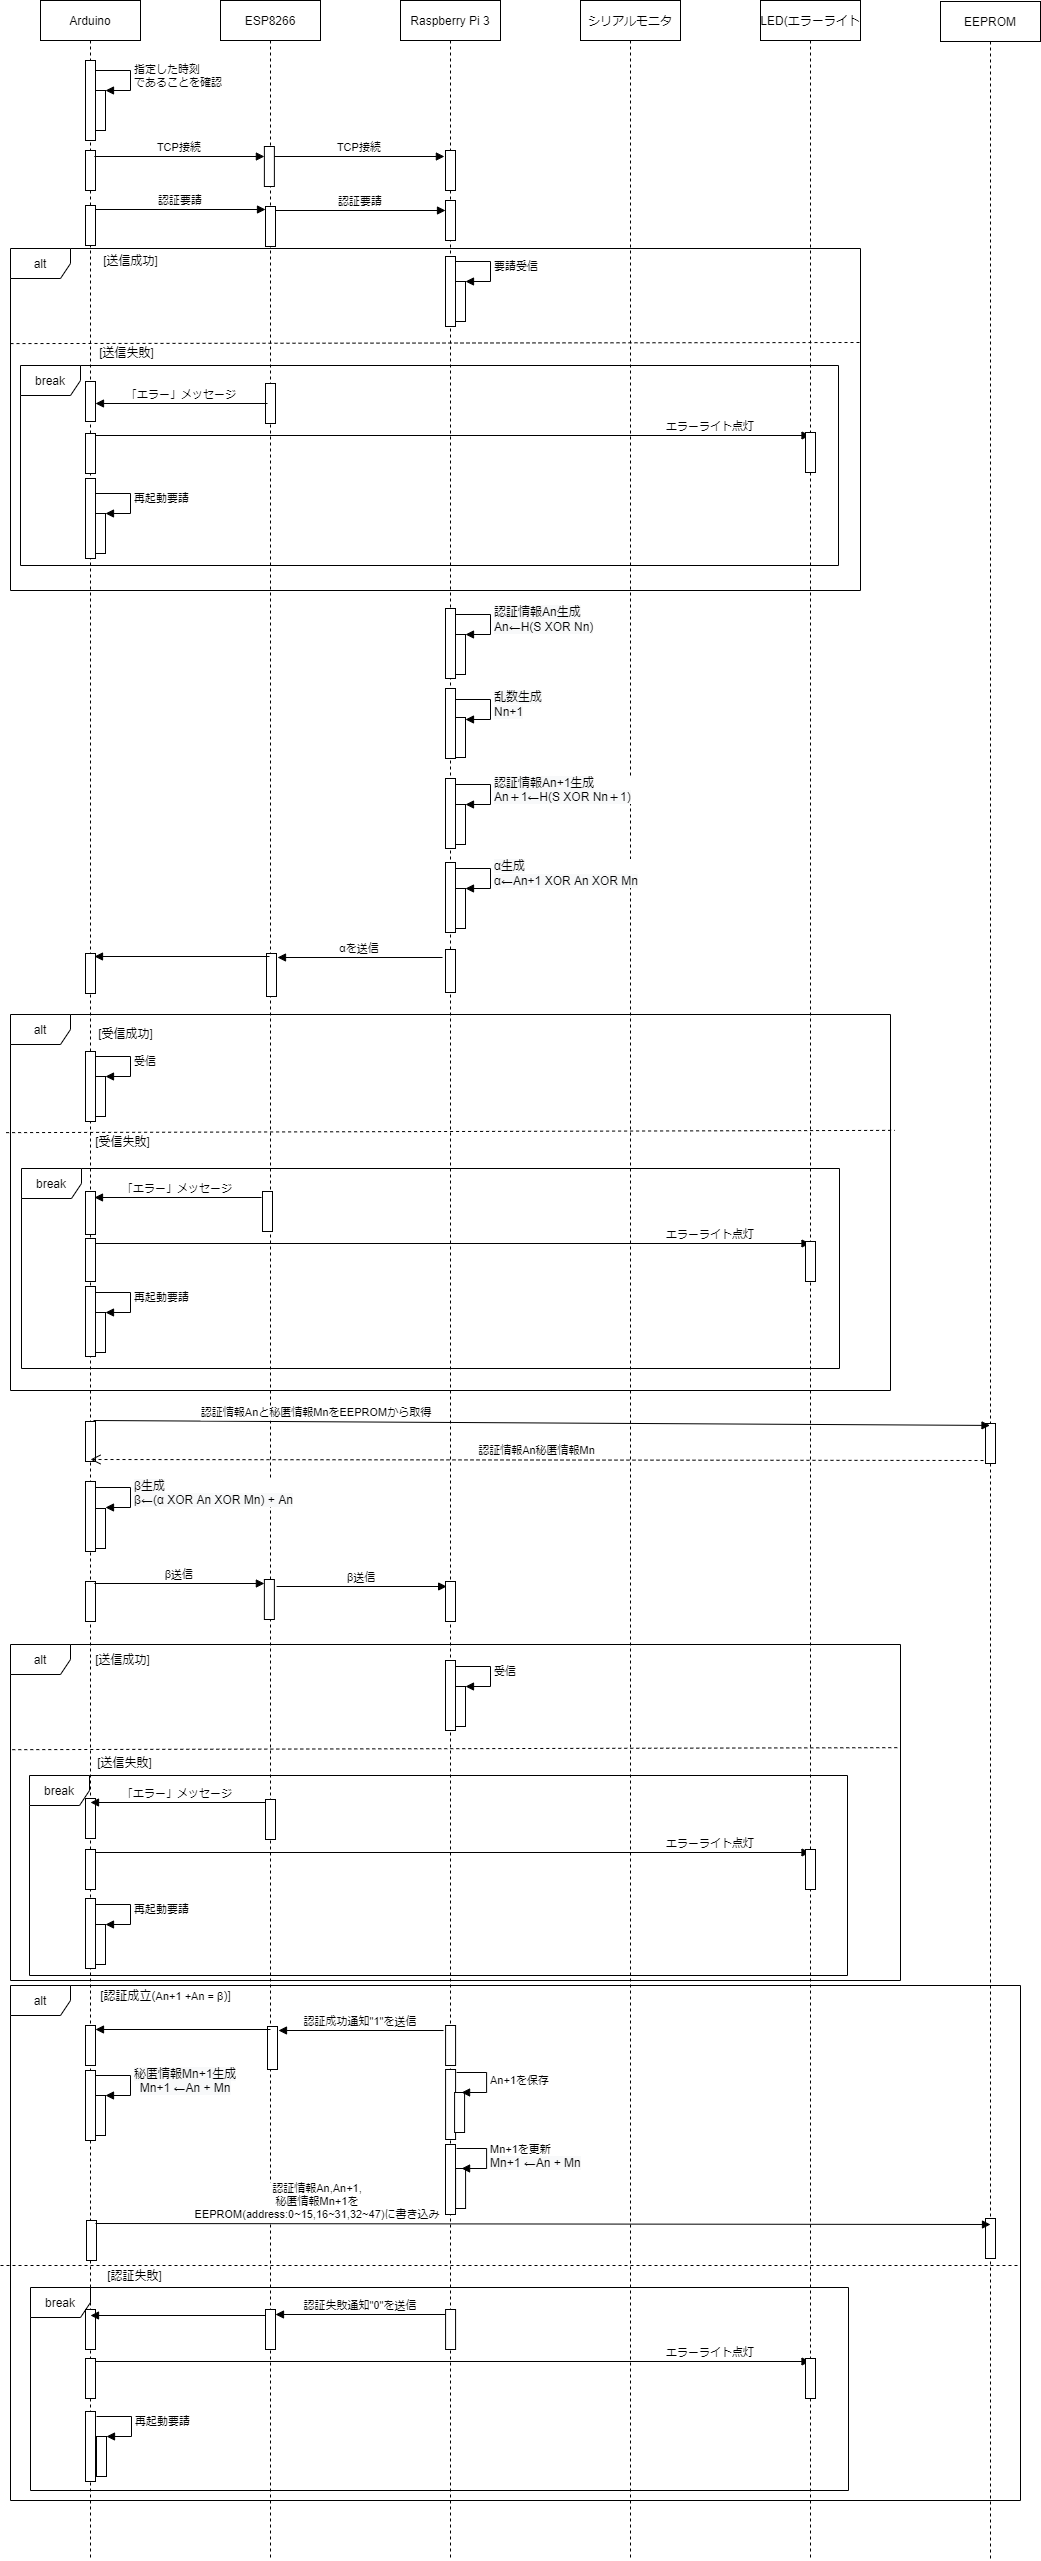
\includegraphics[height=220mm]{ninsyo_sequence.png}
	\caption{認証におけるシーケンス図}
	\label{fig:ninsyo_sequence}
\end{center}
\end{figure}

図\ref{fig:ninsyo_sequence}のシーケンス図では,Arduinoにおける認証に関するクラス間で行われる処理を時系列で表している.
初めに,Arduinoが指定した時刻になると,Raspberry Piに対してTCP接続を行い,認証要請を送信する.
認証要請が送信成功すれば以降の処理に進み,
送信失敗であれば通信モジュールであるESP8266からエラーメッセージがArduinoに対して送信され,
Arduinoの赤LEDが点滅し,利用者に対して再起動するように求める.
次に,Raspberry Piから$\alpha$を受信する.この時,受信が失敗すれば,
Arduinoの赤LEDが点滅し,利用者に対して再起動するように求める.
そして,ArduinoのEEPROMに書き込まれている認証情報と秘匿情報を読み出して,
$\beta$を生成し,Raspberry Piへ送信する.この時,送信が失敗すれば,
Arduinoの赤LEDが点滅し,利用者に対して再起動するように求める.
次に,認証結果をRaspberry Piから受信する.
認証成功なら"1"を受信して秘匿情報を生成し,更新した認証情報と秘匿情報をEEPROMに書き込む.
認証失敗なら"0"を受信して,Arduinoの赤LEDが点滅し,利用者に対して再起動するように求める.

\begin{figure}[H]
\begin{center}
	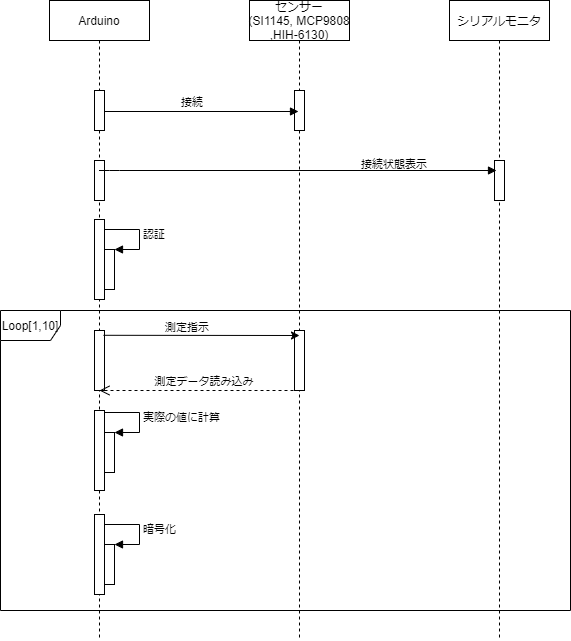
\includegraphics[height=100mm]{sensor_sequence.png}
	\caption{センシングデータ取得におけるシーケンス図}
	\label{fig:sensor_sequence}
\end{center}
\end{figure}

図\ref{fig:sensor_sequence}のシーケンス図では,
Arduinoにおけるセンシングデータ取得に関するクラス間で行われる処理を時系列で表している.
初めに,Arduinoは接続されているセンサと接続を行い,
確認のためにシリアルモニタへセンサとの接続状態を表示する.
次に,認証完了後,Arduinoはセンサへ測定指示を出して測定値を取得する.
取得した測定値を実際の値へと変換するために計算を行う.
計算後の値をセンシングデータとし,そのセンシングデータを利用して暗号化通信を行う.
図\ref{fig:sensor_sequence}に書かれているLoop[1,10]の部分では,10回の繰り返し処理が行われる.

\begin{figure}[H]
\begin{center}
	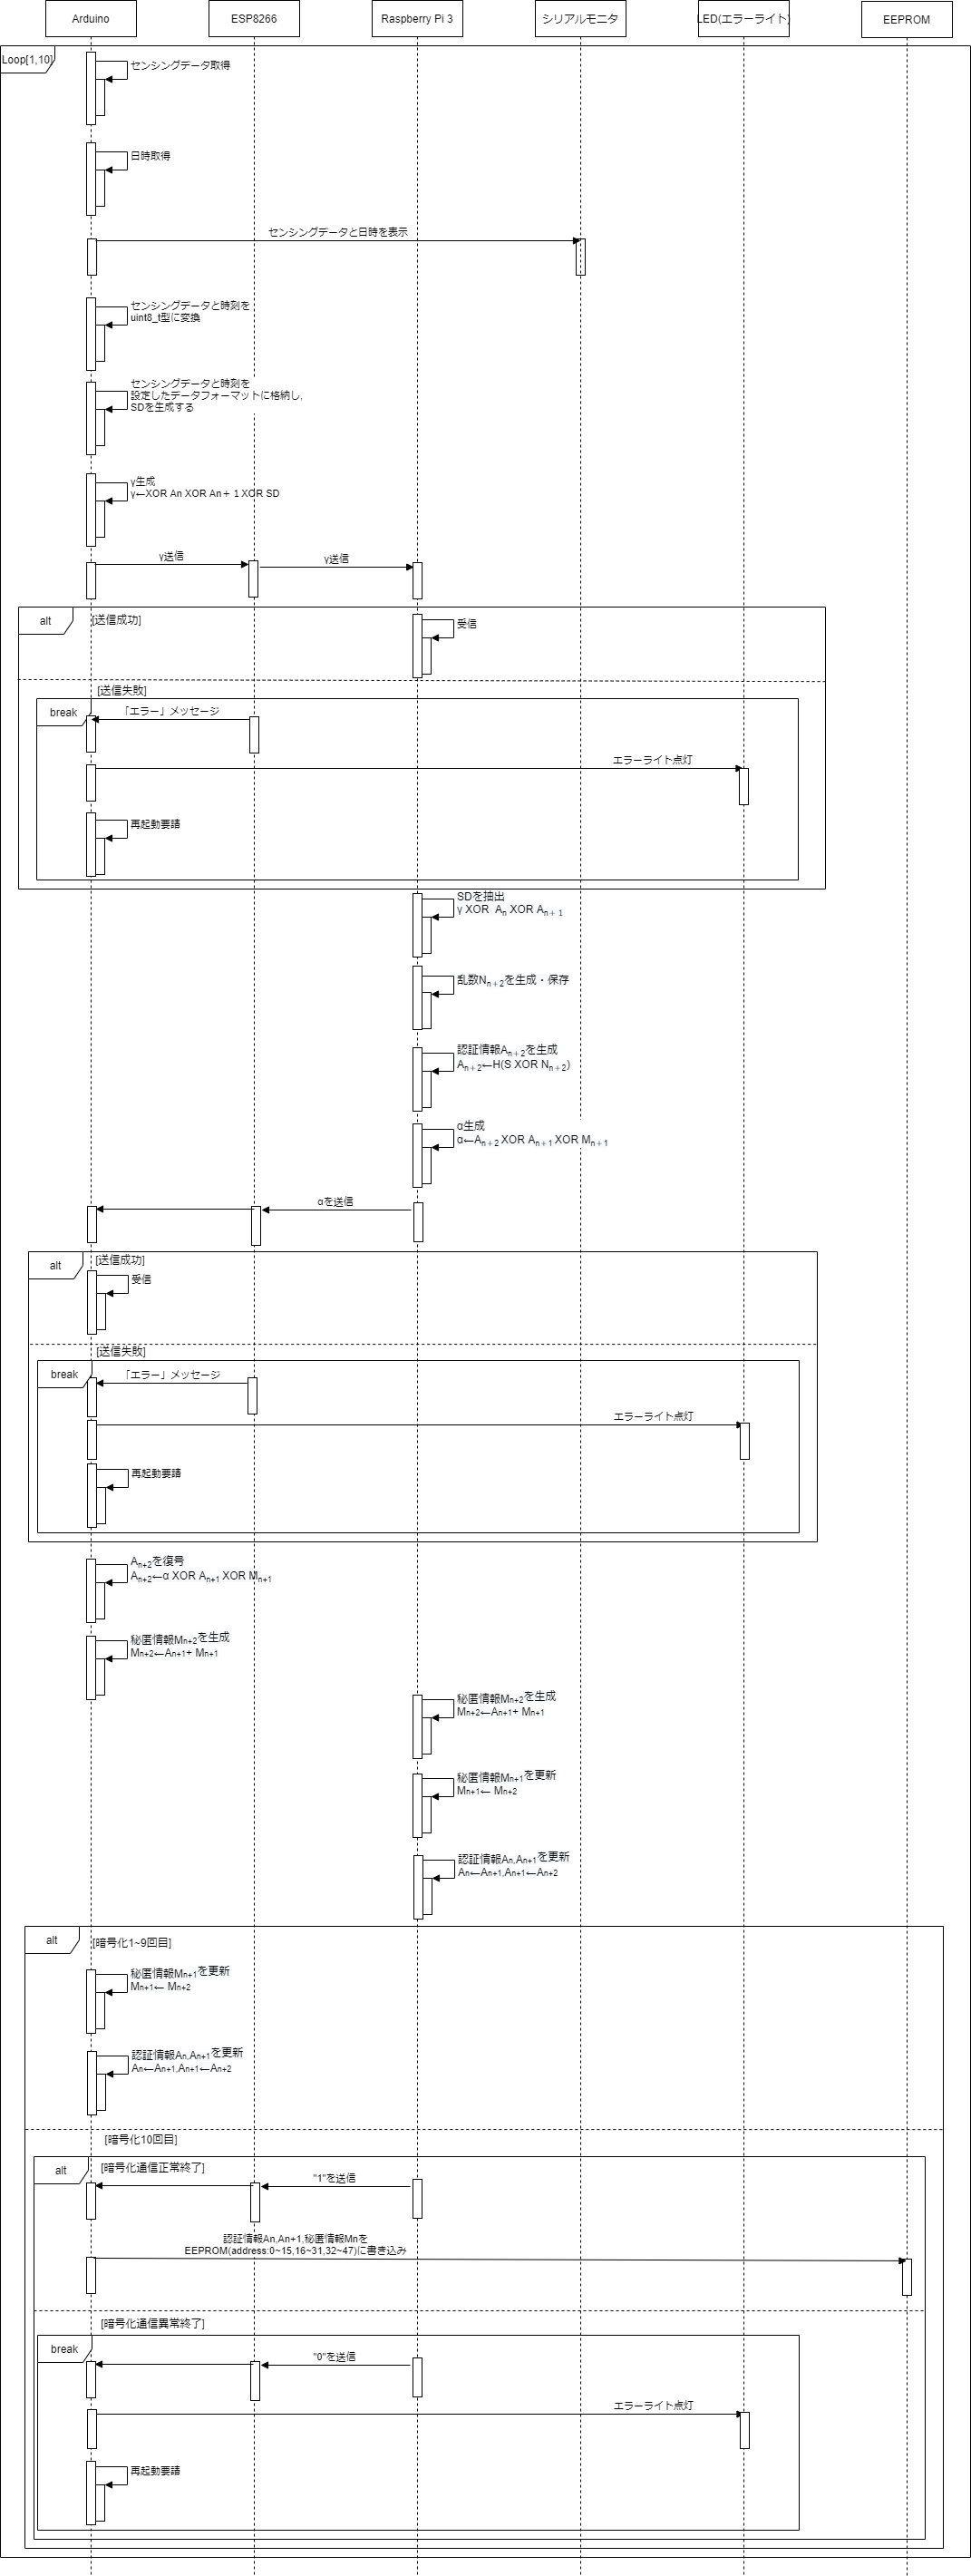
\includegraphics[height=200mm]{ango_sequence.png}
	\caption{暗号化通信におけるシーケンス図}
	\label{fig:ango_sequence}
\end{center}
\end{figure}

図\ref{fig:ango_sequence}のシーケンス図では,
Arduinoにおける暗号化通信に関するクラス間で行われる処理を時系列で表している.
初めに,Arduinoはセンシングデータとセンシングデータを取得した日時を取得する.
そして,取得したセンシングデータと日時をシリアルモニタに表示する.
次に,取得したセンシングデータと日時をunsigned char型へ変換して,データフォーマットに格納し$SD$を生成する.
そして,生成した$SD$を利用して$\gamma$を生成し,Raspberry Piへ送信する.この時,送信が失敗すれば,
Arduinoの赤LEDが点滅し,利用者に対して再起動するように求める.
次に,Raspberry Piから$\alpha$を受信する.この時,受信が失敗すれば,
Arduinoの赤LEDが点滅し,利用者に対して再起動するように求める.
受信した$\alpha$から次回認証情報を復号し,その後,次回秘匿情報を生成する.
最後に,認証情報と秘匿情報の更新を行う.
暗号化通信が1から9回目の場合は,認証情報と秘匿情報を格納している配列を更新する.
暗号化通信が10回目の場合,正常に暗号化通信が終了した時はRaspberry Piから"1"を受信し,
更新した認証情報と秘匿情報をEEPROMに書き込む.
暗号化通信が正常に終了しなかった時は,Raspberry Piから"0"を受信して,
Arduinoの赤LEDが点滅し,利用者に対して再起動するように求める.

%%\begin{figure}[h]
%%\begin{center}
%%	\includegraphics[height=40mm]{syosai_class.eps}
%%	\caption{クラス図}
%%\end{center}
%%\end{figure}

\subsection{データフォーマット}
暗号化通信の際に,$\gamma \leftarrow SD \oplus  A_{n+1} \oplus A_n$の演算によって$\gamma$を生成する.
$\gamma$の生成には$SD$が必要となり,この$SD$にはセンシングデータとセンシングデータを取得した日時が格納されている.
ArduinoとRaspberry Pi間では,基本的にunsigned char型の128bit配列でデータの送受信が行われるため,
センシングデータと日時をunsigned char型の16byte(128bit)配列$SD$に格納するためにデータフォーマットを作成した.作成したデータフォーマットを図\ref{fig:format}に示す.
まず,センシングデータはfloat型で取得される.float型は32bitであることから,センシングデータのビット列は配列$SD$[0]から$SD$[3]に格納する.
次に,日時の内容は年,月,日,時,分,秒である.年はint型の16bitで取得され,月,日,時,分,秒はそれぞれint型の8bitで取得される.
このことから,年のビット列は配列$SD$[4]から$SD$[5]に格納し,月のビット列は配列$SD$[6],日のビット列は配列$SD$[7],
時のビット列は配列$SD$[8],分のビット列は配列$SD$[9],秒のビット列は配列$SD$[10]に格納される.
残りの配列$SD$[11]から$SD$[15]には乱数を設定し格納する.

\begin{figure}[H]
\begin{center}
	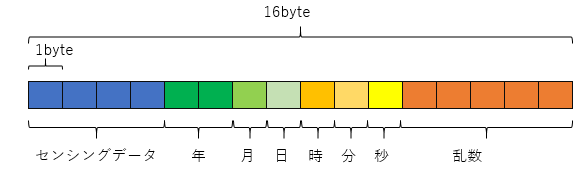
\includegraphics[height=30mm]{format.png}
	\caption{センシングデータと取得日時を格納する際のデータフォーマット}
	\label{fig:format}
\end{center}
\end{figure}

\section{テスト項目の作成}
本節では,本研究で作成した単体テスト項目と結合テスト項目,総合テスト項目について説明する.
\subsection{単体テスト項目}
単体テストではV字開発モデルに従って,詳細設計を参考し表\ref{tab:tantai_komoku}のテスト項目を作成した.
\begin{table}[H]
\centering
\caption{単体テスト項目}
\label{tab:tantai_komoku}
\scalebox{0.8}{
\begin{tabular}{|c|l|} \hline
 機能枠&確認内容\\ \hline\hline
 \multirow{2}{*}{通信モジュールとの接続} & 
  \shortstack[l]{
   ArduinoとESP8266を接続した時,ESP8266との接続が\\
   確認できたら,シリアルモニタに"ESP8266 OK"と表示\\
   される.}\\ \cline{2-2}
 & \shortstack[l]{
   ArduinoとESP8266を接続しなければ,ESP8266との\\
   接続が確認できず,赤LEDが点滅する.}\\ \hline
 Wi-Fi接続 &
   \shortstack[l]{
   Wi-Fiとの接続ができれば,シリアルモニタに"connect\\
   success"と 表示される.}\\ \hline
 UDP接続 &
   \shortstack[l]{
   IPアドレス"ntp.nict.jp",ポート番号"123"へUDP接続が\\
   成功すれば,時刻同期処理が開始される.}\\ \hline
 TCP接続 &
   \shortstack[l]{
   IPアドレス"192.168.2.110"、ポート番号"49152"へTCP\\
   接続が成功すれば, シリアルモニタに"create tcp ok"\\
   と表示される.}\\ \hline 
 \multirow{3}{*}{センサ} &
   Arduinoとセンサが接続している.\\ \cline{2-2}
 & \shortstack[l]{
   Arduinoとセンサが接続されていなければ赤LEDが点滅\\
   する.}\\ \cline{2-2}
 & センシングデータを取得する.\\ \hline
 時刻取得 &
   \shortstack[l]{
   センシングデータを取得した時点の年,月,日,時,分,秒\\
   を取得する.}\\ \hline
 \multirow{2}{*}{認証の際の$\beta$の演算} &
   \shortstack[l]{
   $\alpha \oplus A_n \oplus M_n$の演算結果が正しい.演算結果は128bit\\
   である.}\\ \cline{2-2}
 & \shortstack[l]{
   $\beta \leftarrow (\alpha \oplus A_n \oplus M_n )+A_n$の演算結果が正しい.\\
   演算結果は128bitである.}\\ \hline
 \shortstack[l]{ 
 認証の際の\\
 次回秘匿情報\\
 の計算} &
   \shortstack[l]{
   $M_{n+1} \leftarrow A_n + M_n$の演算が正しい.\\
   演算結果は128bitである.} \\ \hline
 \shortstack[l]{
 認証成功時の\\
 認証情報$A_n$,$A_{n+1}$,\\
 秘匿情報$M_n$の更新}
 & \shortstack[l]{
   n回目認証成功時の$A_n$,$A_{n+1}$,$M_{n+1}$をEEPROMのアドレス\\
   0-15,16-31,32-47にそれぞれ書き込む.}\\ \hline
 $SD$の生成 &
   \shortstack[l]{
   float型(32bit)センサ値と,int型(16bit)の年,int$8_t$型(8bit)\\
   の月,日,時,分,秒をunsigned char型の128bit配列に格納\\
   される.}\\ \hline
\shortstack[l]{
 暗号化通信の際の\\
$\gamma$の演算}&
   \shortstack[l]{
   $\gamma \leftarrow SD \oplus A_{n+1} \oplus A_n$ の演算結果が正しい.\\
   演算結果は128bitである.}\\ \hline
 \shortstack[l]{
 暗号化通信の際の\\
 認証情報$A_{n+2}$の演算} &
   \shortstack[l]{  
   $A_{n+2} \leftarrow \alpha \oplus A_{n+1} \oplus M_{n+1}$の演算結果が正しい.\\
   演算結果は128bitである.}\\ \hline
 \shortstack[l]{ 
 暗号化通信の際の\\
 次回秘匿情報の計算} &
   \shortstack[l]{
   $M_{n+2} \leftarrow A_{n+1} + M_{n+1}$の演算が正しい.演算結果は128bit\\
   である.}\\ \hline
 \shortstack[l]{ 
 暗号化通信の際の\\
 認証情報,\\
 秘匿情報の更新} &
   \shortstack[l]{   
   10回目暗号化終了時の$A_n$,$A_{n+1}$,$M_{n+1}$をEEPROMの\\
   アドレス0-15,16-31,32-47それぞれ書き込む.}\\ \hline
\end{tabular}
}
\end{table}

\subsection{結合テスト項目}
結合テストではV字開発モデルに従って,基本設計を参考し表\ref{tab:ketugo_komoku}のテスト項目を作成した.
Arduinoはユーザー,Raspberry Piはサーバーと定義する.


\begin{table}[H]
\centering
\caption{結合テスト項目}
\label{tab:ketugo_komoku}
\scalebox{0.8}{
\begin{tabular}{|c|l|} \hline
 機能枠&確認内容\\ \hline\hline
 \multirow{5}{*}{認証} &
   認証要請の送受信を行う.\\ \cline{2-2}
 & \shortstack[l]{
   認証の際,$\alpha$の送受信を行い,サーバーが送信したデータと,\\
   ユーザーが受信したデータが一致している.}\\ \cline{2-2}
 & \shortstack[l]{
   認証の際,$\beta$の送受信を行い,ユーザーが送信したデータと,\\
   サーバーが受信したデータが一致している.}\\ \cline{2-2}
 & 認証結果の送受信を行う.\\ \cline{2-2}
 & \shortstack[l]{
   ユーザーで演算した認証情報$A_{n+1}$,秘匿情報$M_{n+1}$と,サーバーで\\
   演算した認証情報$A_{n+1}$,秘匿情報$M_{n+1}$が一致している.}\\ \hline
 \multirow{4}{*}{暗号化通信} &
   \shortstack[l]{
   $\gamma$の送受信を行い,ユーザーが送信したデータと,サーバーが受信\\
   したデータが一致している.}\\ \cline{2-2}
 & \shortstack[l]{
   ユーザーが取得したセンシングデータと日時が,データベースに\\
   保存されたセンシングデータと日時と一致している. }\\ \cline{2-2}
 & \shortstack[l]{
   暗号化通信の際,$\alpha$の送受信を行い,サーバーが送信したデータと,\\
   ユーザーが受信したデータが一致している.}\\ \cline{2-2}
 & \shortstack[l]{
   暗号化通信終了後,ユーザーとサーバーがそれぞれ演算を行った\\
   認証情報$A_n$と秘匿情報$M_n$が一致している.}\\ \hline
 \end{tabular}
}
\end{table}

\subsection{総合テスト項目}
総合テストではV字開発モデルに従って,要件定義を参考し表\ref{tab:sogo_komoku}のテスト項目を作成した.
Arduinoはユーザー,Raspberry Piはサーバーと定義する.
\begin{table}[H]
\centering
\caption{総合テスト項目}
\label{tab:sogo_komoku}
\scalebox{0.8}{
\begin{tabular}{|c|l|} \hline
 機能枠&確認内容\\ \hline\hline
 \multirow{12}{*}{認証}
 & ユーザーは起動後,1度時刻同期を行う.\\ \cline{2-2}
 & ユーザーが指定した時間に認証要請を送信する.\\ \cline{2-2}
 & \shortstack[l]{
   複数のユーザーは同時刻に認証要請を送信するので,一台の認証\\ 
   が終了するまで,その他のユーザーは待機状態になる.}\\ \cline{2-2}
 & ユーザーが認証処理を行っている.\\ \cline{2-2}
 & ユーザーが認証結果をモニタに表示している.\\ \cline{2-2}
 & \shortstack[l]{ 
   認証が成功した場合,ユーザーがSAS-L2に基づいた\\
   暗号化通信を行う.}\\ \cline{2-2}
 & \shortstack[l]{
   認証が失敗した場合,ユーザーはコネクションを切断して認証要請送信\\
   から再度開始する.}\\ \cline{2-2}
 & サーバーが起動したら,受信待ち状態になる.\\ \cline{2-2}
 & サーバーが認証要請受信後,認証処理を行っている.\\ \cline{2-2}
 & サーバーが認証結果をモニタに表示している.\\ \cline{2-2} 
 & \shortstack[l]{ 
   認証が成功した場合,サーバーがSAS-L2に基づいた暗号化通信を\\
   行う.}\\ \cline{2-2}
 & \shortstack[l]{
   認証が失敗した場合,サーバーはコネクションを切断して認証要請の\\
   待ち状態となる.}\\ \hline
 \multirow{9}{*}{暗号化通信}
 & ユーザーはセンシングデータを取得する.\\ \cline{2-2}
 & \shortstack[l]{
   ユーザーは,シリアルモニタに取得したセンシングデータ\\
   とセンシングデータ取得日時を表示する.}\\ \cline{2-2}
 & \shortstack[l]{
   ユーザーはセンシングデータと日時を暗号化して\\
   サーバーへ送信する.}\\ \cline{2-2}
 & ユーザーは暗号化通信を10回行う.\\ \cline{2-2}
 & ユーザーは暗号化通信後,コネクションを切断する.\\ \cline{2-2}
 & サーバーはセンシングデータと日時を復号する.\\ \cline{2-2}
 & \shortstack[l]{
   サーバーはセンシングデータと取得日時を保存する際に,\\
   ユーザーごとのテーブルに分けて保存する.} \\ \cline{2-2}
 & サーバーは暗号化通信を10回行う.\\ \cline{2-2}
 & \shortstack[l]{
  サーバーは暗号化通信後,コネクションを切断し\\
   認証要請待ち状態となる.}\\ \hline
\multirow{3}{*}{通信}
& ユーザーで,何らかのエラーが発生した場合,赤LEDを点滅させる.\\ \cline{2-2}
& \shortstack[l]{
   サーバーは5秒以上データを受信できなければ,\\
   コネクションを切断して認証要請受信の待機状態となる.}\\ \cline{2-2}
& \shortstack[l]{
   3台のユーザーが同時刻に認証要請を送信した場合,3台のユーザーとの\\
   通信が10秒以内に完了する.}\\ \hline
\end{tabular}
}
\end{table}
